% !TEX encoding = UTF-8 Unicode
\documentclass[a4paper,12pt]{book}

\setlength{\headheight}{1.1\baselineskip}
 
\usepackage[utf8]{inputenc}
\usepackage[spanish]{babel}

\usepackage{geometry}
\usepackage[sc]{mathpazo}

\usepackage{amsmath}

\usepackage[usenames,dvipsnames]{color} 
\usepackage{hyperref}
\usepackage{alltt}

% Para footer con páginas
\usepackage{scrpage2}
\usepackage{lastpage}

% Para insertar imágenes y ubicarlas
\usepackage{graphicx}
\usepackage{placeins}

% Para insertar código
\usepackage{xcolor}
\usepackage{listings}

\usepackage[T1]{fontenc} %%%key to get copy and paste for the code!

\usepackage{amssymb,amsmath}

% Source Code
\usepackage{color}
\usepackage{textcomp}
\usepackage{listings}
\usepackage{amsfonts}
\usepackage{courier}

\definecolor{source}{gray}{0.9}

% my comment style
\newcommand{\myCommentStyle}[1]{{\ttfamily\footnotesize\color{gray!100!white} #1}}

% my string style
\newcommand{\myStringStyle}[1]{{\ttfamily\footnotesize\color{violet!100!black} #1}}

% my symbol style
\newcommand{\mySymbolStyle}[1]{{\ttfamily\footnotesize\color{violet!100!black} #1}}

% my keyword style
\newcommand{\myKeywordStyle}[1]{{\ttfamily\footnotesize\color{green!70!black} #1}}

% my global style
\newcommand{\myGlobalStyle}[1]{{\ttfamily\footnotesize\color{blue!100!black} #1}}

% my number style
\newcommand{\myNumberStyle}[1]{{\ttfamily\footnotesize\color{brown!100!black} #1}}

\lstset{
language={},
% characters
tabsize=3,
escapechar={!},
keepspaces=true,
breaklines=true,
alsoletter={\#},
literate={\$}{{{\$}}}1,
breakautoindent=true,
columns=fullflexible,
showstringspaces=false,
% background
frame=single,
aboveskip=1em, % automatic space before
framerule=0pt,
basicstyle=\ttfamily\footnotesize\color{black},
keywordstyle=\myKeywordStyle,% keyword style
commentstyle=\myCommentStyle,% comment style
frame=single,%
backgroundcolor=\color{source},
% numbering
stepnumber=1,
numbersep=10pt,
numberstyle=\tiny,
numberfirstline=true,
% caption
captionpos=b,
% formatting (html)
moredelim=[is][\bfseries]{<b>}{</b>},
moredelim=[is][\textit]{<i>}{</i>},
moredelim=[is][\underbar]{<u>}{</u>},
moredelim=[is][\color{red}\uwave]{<wave>}{</wave>},
moredelim=[is][\color{red}\sout]{<del>}{</del>},
moredelim=[is][\color{blue}\underbar]{<ins>}{</ins>},
% smalltalk stuff
morecomment=[s][\myCommentStyle]{"}{"},
%    morecomment=[s][\myvs]{|}{|},
morestring=[b][\myStringStyle]',
moredelim=[is][]{<sel>}{</sel>},
moredelim=[is][]{<rcv>}{</rcv>},
moredelim=[is][\itshape]{<symb>}{</symb>},
moredelim=[is][\scshape]{<class>}{</class>},
morekeywords={true,false,nil,self,super,thisContext},
identifierstyle=\idstyle,
}

\makeatletter
\newcommand*\idstyle[1]{%
\expandafter\id@style\the\lst@token{#1}\relax%
}
\def\id@style#1#2\relax{%
\ifnum\pdfstrcmp{#1}{\#}=0%
% this is a symbol
\mySymbolStyle{\the\lst@token}%
\else%
\edef\tempa{\uccode`#1}%
\edef\tempb{`#1}%
\ifnum\tempa=\tempb%
% this is a global
\myGlobalStyle{\the\lst@token}%
\else%
\the\lst@token%
\fi%
\fi%
}
\makeatother


%\newcommand{\ct}{\lstinline[backgroundcolor=\color{white}]}
%\newcommand{\needlines}[1]{\Needspace{#1\baselineskip}}
\newcommand{\lct}{\texttt}

\lstnewenvironment{code}{%
    \lstset{%
    % frame=lines,
    frame=single,
    framerule=0pt,
    mathescape=false
    }%
    \noindent%
    \minipage{\linewidth}%
}{%
    \endminipage%
}%


\lstnewenvironment{codeWithLineNumbers}{%
    \lstset{%
    % frame=lines,
    frame=single,
    framerule=0pt,
    mathescape=false,
    numbers=left
    }%
    \noindent%
    \minipage{\linewidth}%
}{%
    \endminipage%
}%

%For simple inlined code
\newcommand{\ct}{\texttt}

%utiles e.g., i.e., c.f.
\usepackage{xspace}
\newcommand{\eg}{\emph{e.g.,}\xspace}
\newcommand{\ie}{\emph{i.e.,}\xspace}
\newcommand{\cf}{\emph{c.f.}\xspace}

%For comments
\usepackage{ifthen}
\newboolean{showcomments}
\setboolean{showcomments}{true}
\ifthenelse{\boolean{showcomments}}
  {\newcommand{\bnote}[2]{
	\fbox{\bfseries\sffamily\scriptsize#1}
    {\sf\small$\blacktriangleright$\textit{#2}$\blacktriangleleft$}
    % \marginpar{\fbox{\bfseries\sffamily#1}}
   }
   \newcommand{\cvsversion}{\emph{\scriptsize$-$Id: macros.tex,v 1.1.1.1 2007/02/28 13:43:36 bergel Exp $-$}}
	\newcommand{\del}[1]{\bnote{Remove}{\textcolor{gray} #1}}
  }
  {\newcommand{\bnote}[2]{}
   \newcommand{\cvsversion}{}
	\newcommand{\del}[1]{}
  } 

\newcommand{\gp}[1]{\bnote{Guille}{#1}}
\newcommand{\fd}[1]{\bnote{Fer}{#1}}

\newtheorem{definition}{Definición}

\newenvironment{codeNonSmalltalk}
{\begin{alltt}\ttfamily}
{\end{alltt}\normalsize}

% Para insertar boxes
\usepackage[framemethod=TikZ]{mdframed}
\mdfdefinestyle{BoxFrame}{%
    linecolor=black,
    outerlinewidth=1pt,
    roundcorner=20pt,
    innertopmargin=\baselineskip,
    innerbottommargin=\baselineskip,
    innerrightmargin=20pt,
    innerleftmargin=20pt,
    backgroundcolor=gray!30!white}

\renewcommand{\labelitemi}{$\bullet$}
\renewcommand{\labelitemii}{$\cdot$}
\renewcommand{\labelitemiii}{$\diamond$}
\renewcommand{\labelitemiv}{$\ast$}  

\ifoot[]{}
\cfoot{\thepage\ of \pageref{LastPage} }
\ofoot[]

\pagestyle{scrplain}

\vspace{0.1in}

\definecolor{dkgreen}{rgb}{0,0.6,0}
\definecolor{gray}{rgb}{0.5,0.5,0.5}
\definecolor{mauve}{rgb}{0.58,0,0.82}

\begin{document}

\chapter{Herencia}
Las colecciones son un concepto importante y poderoso al diseñar con objetos. En este capítulo veremos cómo
se modela el conocimiento de un conjunto de referencias de un objeto y su utilización para resolver un problema
concreto.

\tableofcontents

\section{Introducción}

En capítulos precedentes introdujimos el concepto de \emph{clase}: un molde que define la estructura y comportamiento de los objetos creados a partir de ella. Las clases nos ofrecen tanto un marco conceptual como ventajas prácticas: por un lado nos permiten agrupar objetos similares bajo una misma abstracción, dándoles un nombre común (el nombre de la clase), y por otro lado nos permiten definir una única vez el comportamiento de un objeto y reutilizarlo en varios objetos. Por ejemplo, podemos podemos definir una clase \ct{Heroe} que permita desplazar nuestros héroes entre distintos casilleros de la siguiente manera:

\begin{code}
Object subclass: #Heroe
	instanceVariableNames: ''.
	
Heroe >> desplazarseA: unCasillero
    unCasillero recibirHeroe: self.
\end{code}

Consideremos ahora que queremos introducir distintas \emph{especies} de héroes: arqueros y guerreros. Arqueros y guerreros son héroes que van a participar en distintas batallas épicas y por lo tanto deben poder hacer daño. Además, tanto arqueros como guerreros poseen, obviamente, distintas características de combate que podemos representar en código utilizando distintas clases \ct{Arquero} y \ct{Guerrero}:

\begin{code}
Object subclass: #Arquero
	instanceVariableNames: 'flecha'.
	
Arquero >> danoCausado
    ^ flecha poder + self modificadorDestreza.
    
Object subclass: #Guerrero
	instanceVariableNames: 'arma'.
	
Guerrero >> danoCausado
    ^ arma poder + self modificadorFuerza.
\end{code}

Usar distintas clases para guerreros y arqueros nos permite definir distintos comportamientos para cada uno de ellos. Sin embargo, nuestros nuevos héroes ya no comparten el comportamiento que definimos anteriormente en nuestra clase \ct{Heroe}. Para solucionar este problema, este capítulo introduce el concepto de \textbf{herencia}. La herencia es una relación entre clases que permite definir super-clasificaciones y sub-clasificaciones de objetos, generar distintos niveles de abstracción y compartir comportamiento entre distintas clases. Estos distintos niveles de abstracción llevan a la aparición de clases concretas y clases abstractas. Finalmente este capítulo discute distintos criterios de aplicación de herencia.

\section{Clasificando Objetos con Herencia}

Previamente estudiamos cómo las clases nos permiten clasificar objetos similares. Todos los objetos de la misma clase tienen comportamiento y estructura similar. Por ejemplo, Diego y Jorge son dos guerreros que poseen un arma y atacan de la misma manera. De la misma manera podemos encontrar otras clasificaciones de objetos que tienen comportamientos y/o estructuras distintas como son los arqueros en nuestro ejemplo.

Pese a que arqueros y guerreros pertenecen claramente a distintas clases de objetos dado que exhiben distinto comportamiento, ambos tienen también algunas características en común ya que ambos conforman nuestro grupo de héroes. La Figura \ref{fig:herencia_venn} muestra como se relacionan nuestros distintos objetos (Diego, Jorge y Sergio) utilizando un diagrama de Venn. En la figura vemos que Diego y Jorge está incluidos dentro del conjunto de guerreros y Sergio está incluido en el conjunto de arqueros. Ambos conjuntos están incluidos en un conjunto más grande y más abstracto: el conjunto de héroes. Si consideramos que los conjuntos distintos conjuntos definen clases en nuestro programa, entonces decimos que la clase \ct{Guerrero} son subclases de la clase \ct{Héroe}. De manera más general podemos definir esta relación de la siguiente manera:

\begin{definition}\textbf{Superclase.} 
Una clase $C1$ es superclase de una clase $C2$ si $C2$ define un subconjunto de $C1$.
\end{definition}

De manera recíproca, podemos definir la relación de subclase:

\begin{definition}\textbf{Subclase.} 
Una clase $C1$ es subclase de $C2$ si $C2$ es superclase de $C1$.
\end{definition}

\begin{figure}
    \centering
    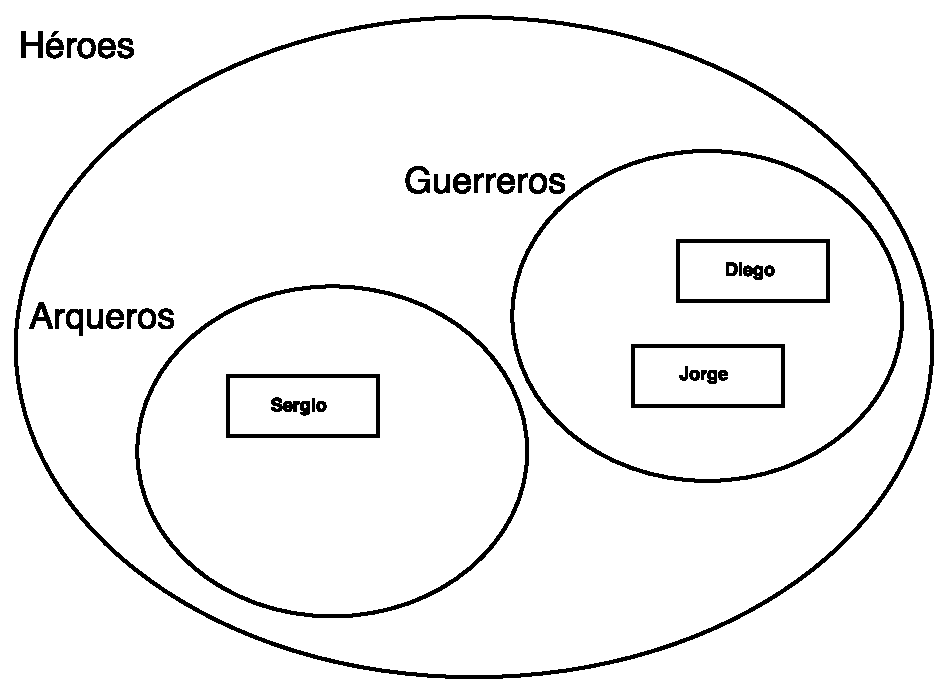
\includegraphics[width=0.6\textwidth]{figures/venn_clasificacion.pdf}
    \caption{Diagrama de Venn presentando las ideas de super-clasificación y sub-clasificaciones en nuestro ejemplo de héroes, guerreros y arqueros.\label{fig:herencia_venn}}
\end{figure}


\subsection{Herencia}

Para representar la relación de sub y superclasificación entre clases usamos \emph{herencia}.
La herencia es una relación entre dos clases donde una clase es superclase de la otra. Decimos que la subclase \emph{hereda} la estructura y el comportamiento de la superclase, permitiéndonos combinar el comportamiento definido en distintas clases. En nuestro ejemplo, podemos decir que un guerrero~(\ie una instancia de la clase \ct{Guerrero}) exhibe el comportamiento de un guerrero~(\ie el comportamiento definido en su clase) y el comportamiento de un héroe~(\ie el comportamiento definido en la superclase de su clase). Más aún, al separar el comportamiento de los héroes en la clase \ct{Héroe}, podemos compartirlo entre distintas clases de héroes.

Podemos ilustrar la relación de herencia en un diagrama de clases tal y como aparece en \autoref{fig:herencia_uml}: una flecha con punta cerrada blanca que se dirige desde una subclase hacia una superclase.\gp{quizás es mejor mostrar un diagrama con una sola clase/subclase} Para efectuar la relación de herencia entre dos clases en Pharo, debemos modificar la definición de la clase como sigue, indicando que la clase \ct{Heroe} posee las subclases \ct{Arquero} y \ct{Guerrero}. 


\begin{code}
Heroe subclass: #Arquero
	instanceVariableNames: 'flecha'.
	
Heroe subclass: #Guerrero
	instanceVariableNames: 'arma'.
\end{code}

\begin{figure}
    \centering
    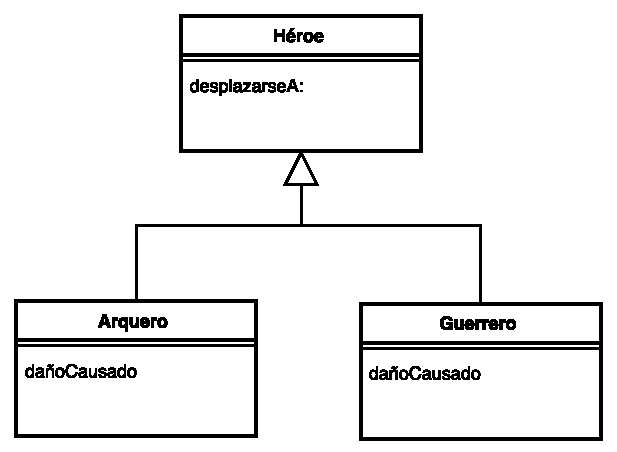
\includegraphics[width=0.5\textwidth]{figures/herencia}
    \caption{Diagrama de clases representando la relación de herencia entre las clases \ct{Héroe}, \ct{Guerreros} y \ct{Arquero}.\label{fig:herencia_uml}}
\end{figure}

\subsection{Herencia de comportamiento}

method lookup nueva version

\subsection{Herencia de atributos}

\subsection{\ct{self} y \ct{super}}


method lookup revisited 2
self vs super

\section{Clases concretas vs clases abstractas}

Al generar superclases sigo perdiendo información, gano en generalidad. Un Ave quizás no
tenga sentido instanciarlo. Si en mi aplicación no voy a instanciar aves (porque representan un
concepto demasiado general) entonces la clase es abstracta.
Diferencia entre Smalltalk y Java:

1) En Smalltalk no tiene sentido crear un ave, aunque podría. La clase es abstracta
cuando no tengo intención de crear instancias de esa clase (porque no tiene sentido).

2) En Java no puedo crear un ave aunque quisiera. La clase es abstracta y el compilador
me impide generar instancias de esa clase. Son dos filosofías distintas.
public abstract class Ave forma parte de la definición misma de clase

ejemplo de herencia con superclase abstracta
ejemplo de herencia con superclase concreta

\section{Criterios para utilizar herencia}
\subsection{Usar Objetos vs Clases}
\subsection{Especializar vs Generalizar}

Otra forma de ver la herencia: subclasificamos un concepto conocido, lo refinamos. Si mi hija
no conoce lo que es una tonina, yo le puedo explicar: “Y… es como un delfín pero negro” (una
especie de … pero que …; mostrando tanto en lo que se parece como en lo que se diferencia). 

Tenemos conceptos conocidos: golondrina, colibrí, torcaza, paloma, gorrión. Muchos de estos
pájaros tendrán cosas en común pero se diferencian en algo…
Una vez que reconocí varios objetos, puedo abstraer una clase. Pierdo información, porque lo
que obtengo es más general (una golondrina genérica, en lugar de esta o aquella golondrina,
que era de color azul y yo llamaba pepita).
Ahora vamos a trabajar con otro tipo de abstracción: tengo varias clases (conceptos) y llego a
una jerarquía de clases de la más general a las más particulares: 

Otra forma de ver la herencia: subclasificamos un concepto conocido, lo refinamos. Si mi hija
no conoce lo que es una tonina, yo le puedo explicar: “Y… es como un delfín pero negro” (una
especie de … pero que …; mostrando tanto en lo que se parece como en lo que se diferencia).

\subsection{subclase vs subtipo}
\subsection{Herencia vs composición}

  
\end{document}
